\textbf{\textit{“Good architecture makes the system easy to understand, easy to develop, easy to maintain, and easy to deploy. The ultimate goal is to minimize the lifetime cost of the system and to maximize programmer productivity.” - Robert C. Martin}} \cite{10}

Software systems grow and change over the time. As a software system changes, the interactions between different system elements lead to complexity. To develop reliable software systems that can overcome this complexity, programmers must implement software systems in a generalized fashion. Software systems written in such a fashion can be considered reliably usable, maintainable, testable, and extendable \cite{15}. This fashion is called software architecture. Martin Fowler defines the software architecture as "the shared understanding that the expert developers have of the system design" \cite{16}. The formal definition of software architecture is "the set of significant decisions about the organization of a software system, the selection of structural elements and their interfaces by which the system is composed, together with their behaviour as specified in the collaborations among those elements, the composition of these elements into progressively larger subsystems, and the architectural style that guides this organization -- these elements and their interfaces, their collaborations, and their composition" \cite{17}. The role of software architecture in software development can be elaborated under the six major aspects. Those aspects can be listed as follows \cite{25}:
\begin{itemize}
    \item \textbf{Understanding:} Software architecture simplifies the understanding and improves the readability of software systems.
    \item \textbf{Reuse:} Software architecture facilitates  the code reuse between the components.
    \item \textbf{Construction:} Software describes the components of the system and dependencies between those components.
    \item \textbf{Evolution:} Software architecture helps developers to understand the consequences of changes more accurately and describes the concerns of the software systems.
    \item \textbf{Analysis:} Software architecture enables analyzing the system consistency, compliance with restrictions imposed by the architecture, and with the quality attributes.
    \item \textbf{Management:} Assessment of software architecture facilitates understanding of risks, requirements, and implementation strategies.
\end{itemize}

When the list above is examined, the effects of these roles on the maintainability of software systems are obvious. This situation is also clearly demonstrated in a study on the architecture of Android applications. A related study that is conducted on the topic of Android application architecture had revealed that the top quality requirement for Android application architecture is maintainability \cite{14}. Results can be seen in Fig. \ref{fig:arch_quality_req_ranking}.
\begin{figure}[ht!]
    \centering
    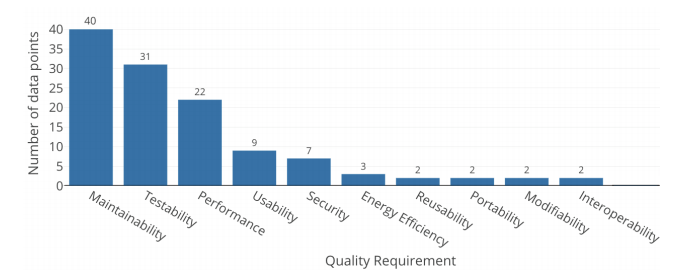
\includegraphics[scale=0.5]{figures/quality_req.png}
    \caption{Quality requirement rankings for Android app architecture \protect\cite{14}}
    \label{fig:arch_quality_req_ranking}
\end{figure}
\FloatBarrier

Also, other quality requirements presented in Fig. \ref{fig:arch_quality_req_ranking}, are in correlation with maintainability. As a consequence, the impact of the architecture on the maintainability of software systems is one of the top aspects that should be considered before starting the development. As Brian Foote quotes, "if you think good architecture is expensive, try bad architecture"\cite{10}.